\documentclass[12pt]{article}
%\linespread{1}
\usepackage[margin=1.0in]{geometry}

\usepackage{amsmath}
\usepackage{amssymb}
\usepackage{multicol}
\usepackage{graphicx}

\title{Distributed Sampled Convex Problems}
\author{David Eckman (dje88) and Calvin Wylie (cjw278)}
\date{}

\begin{document}

%\noindent
\setlength{\parindent}{24pt}

\maketitle

\section*{Abstract}
It is well-known that chance constrained programs are in general intractable because of the non-convexity of the feasible region and the requirement of prior information about the distribution of the uncertain parameters.
Solving a sampled convex program is an appealing way to find solutions that are feasible for the chance constrained program with high probability because these problems are characterized by a finite number of constraints and require only that one can obtain i.i.d. samples of the uncertain parameters.
Existing bounds on the required number of samples may still result in a sampled convex program that is expensive to solve exactly.
We consider obtaining approximate solutions to these sampled convex programs by distributing the constraints across processors and solving smaller subproblems followed by a consensus across processors about the active constraints.
We consider a classical portfolio-optimization problem and study the tradeoffs that arise from this method: including wall-clock time, violation probability, and feasibility probability.

\section*{Introduction}
A typical chance-constrained program \ref{CCP} is given by
\begin{align}\label{CCP}
\begin{split}
\begin{aligned}
    & \underset{x \in \mathcal{X}}{\text{minimize}}
    & & c^T x \\
    & \text{subject to}
    & & \mathbb{P}\{f(x,\delta) \leq 0\} \geq 1-\epsilon.
\end{aligned}
\end{split} \tag{CCP$_\epsilon$}
\end{align}
where $\mathcal{X} \subseteq \mathbb{R}^n$ is compact, $\delta$ is the uncertain parameter, $\mathbb{P}$ is a probability measure on the uncertainty set $\Delta \subseteq \mathbb{R}^d$, and $f:\mathcal{X} \times \Delta \mapsto \mathbb{R}$ is convex in $x$ for any fixed $\delta$.
Chance constrained problems model many real-word applications in areas as diverse as finance, energy, and emergency services.
For example, the parameter $\epsilon$ can represent the acceptable level of risk or a fixed service level requirement.
The difficulty in solving \ref{CCP} comes from the fact that the feasible region is, in general, non-convex and the requirement that one knows the distribution $\mathbb{P}$ a priori.

One method for finding solutions with good performance, which are feasible for \ref{CCP} with high probability is to take $N$ i.i.d. samples $(\delta_i, \ldots, \delta_N)$ from the uncertainty set $\Delta$ according to a probability measure $\mathbb{P}$ and solve the corresponding sampled convex program \ref{SCP}:
\begin{align}\label{SCP}
\begin{split}
\begin{aligned}
    & \underset{x \in \mathcal{X}}{\text{minimize}}
    & & c^T x \\
    & \text{subject to}
    & & f(x,\delta_i) \leq 0 \quad i = 1, \ldots, N.
\end{aligned}
\end{split} \tag{SCP$_N$}
\end{align}
Notice that \ref{SCP} is more tractable than \ref{CCP} since it has a finite number of constraints, a convex feasible region, and we need not explicitly know $\mathbb{P}$ but instead only need to be able to sample from it.

Let $x_N^*$ be the random solution to \ref{SCP} and let $V(x_N^*) = \mathbb{P}\{f(x_N^*, \delta) > 0\}$ be the corresponding violation probability.
To clarify, if $V(x_N^*) \leq \epsilon$, $x_N^*$ is feasible for \ref{CCP} and if $V(x_N^*) > \epsilon$, it is infeasible.
However, $V(x_N^*)$ cannot be explicitly calculated unless we have an analytical form for $\mathbb{P}$.
Instead we often resort to estimating $V(x_N^*)$ via Monte Carlo simulation: obtaining $M$ i.i.d. samples of $\delta$ and calculating
\[ \hat{V}(x_N^*) = \frac{1}{M} \sum_{i = 1}^M \mathbf{1}\{f(x_N^*, \delta_i) > 0\}. \]

Sampled convex programs cannot provide a guarantee that $V(x_N^*) \leq \epsilon$ for a given sample size $N$.
Instead, Calafiore and Campi \cite{campi05} proved that one can bound the number of samples needed to ensure that $\mathbb{P}\{V(x_N^*) > \epsilon\} \leq \beta$.
That is, the optimal solution to \ref{SCP} is feasible for \ref{CCP} with probability greater than $1 - \beta$.
Their bound is $N \geq 1/(\epsilon\beta) - 1$, which was further tightened to choosing $N$ to satisfy
\[ \mathbb{P}^N\{V(x_N^*) > \epsilon\} \leq \binom{N}{d}(1-\epsilon)^{N-d}. \]
in \cite{campi06} and then by Campi and Garatti \cite{campi08} to the solution to a binomial equation:
\[ \mathbb{P}^N\{V(x_n^*) > \epsilon\} = \sum_{i=0}^{d-1} \binom{N}{i} \epsilon^i (1-\epsilon)^{N-i}. \]
Note that all of these bounds are distribution-free.

We are interested in the case when \ref{SCP} is still computationally expensive to solve due to the large number of samples (and therefore constraints) needed to reach a solution that is feasible for \ref{CCP} with high probability.
For example, when $d = 200$, $\epsilon = 0.05$ and $\beta = 1 \times 10^{-5}$ are small, the resulting sample size is $N = 5312$.
With several thousand constraints, existing solution methods for mixed integer programs or semi-definite programs might take too long to run to completion.
For instances such as these, it is possible to decompose \ref{SCP} into smaller sampled convex programs and solving them in parallel.
Because the subproblems are of smaller dimension, they may be solved faster than \ref{SCP}.
However because each subproblem is only considering a subset of the constraints, there is a loss of optimality in solving these problems.
Still the speedup in computational time may be worth the loss of \ref{CCP} feasibility.
In particular, we would like to study how much is lost with respect to \ref{CCP} feasibility by taking the active constraints from the subproblems and solving a final sampled convex program with these constraints.

Even for problems for which $N$ is not too large, but the number of variables $n$ is far too large, this method of parallelism can be applied by taking the dual of \ref{SCP} and then distributing the constraints of the dual across processors.

\section*{Method}

A recent paper \cite{carlone2014} studies solving large-scale convex programs in a distributed fashion.
It assume some topology on the communication network connecting the processors.
Each processor solves a convex program with a subset of the constraints.
It then identifies the active constraints at that solution and passes them to other processors according to the communication network.
Each processor then adds in the incoming constraints to their personal set and resolves their subproblem.
It was proven that after a finite number of iterations, a.s., all processors will reach a consensus about which constraints are active for the solution to the original problem.

The objective in \cite{carlone2014} is to recover the exact solution to the convex program.
However in practice, this procedure would take far too long to run, especially since there is no bound on the number of iterations needed for consensus.
The only instance you would fully run a procedure like this is if the master problem is too large to solve with existing software.

Instead, our method will be a variation of this procedure which only runs for two iterations.
The topology on the processors is that all workers will pass their active constraints to a single master processor, who will then use these constraints to solve another convex program.
Because there are only two iterations, the solutions returned will likely not be the exact solution to \ref{SCP}.
However this approximate solution may be calculated in less time, and thus it may be worth a loss in \ref{CCP} feasibility.
We wish to explore this tradeoff to get a sense of what the best mix would be.

Another tradeoff comes from changing the number of processors.
With more processors, the subproblems are smaller, but the total number of constraints in the second stage problem is larger.
This will impact the wall-clock time of the procedure in two conflicting ways.
The main question will be to determine what the optimal number of processors to use is.

Another way to view the problem is to assume with are willing to use the wall-clock time need to solve \ref{SCP}.
Using that time, what is the best number of processors to use and number of constraints to give to each processor. Because of the time savings from solving smaller problems, we may be able to use more than $N$ samples.

We divide the $N$ samples across $p$ processors and solve each subproblem which has $N/p$ constraints.
We don't want to use so many processors that $N/p < n$.
For each subproblem, we identify the active constraints (of which there should be $n$ unless the problem is degenerate) by checking which $\delta_i$ satisfy $f(x_N^*, \delta_i) = 0$.

\section*{Example Problem}

We consider the classical portfolio optimization problem of selecting an allocation of one dollar over $n$ assets with uncertain payouts $r_i$ for $i = 1, \ldots, n$.
Of these assets, we assume that the $n$th asset has a fixed payout (it might, for example, represent a bond with a certain return).
Our objective is to maximize the value-at-risk (VaR) at a risk level of $\epsilon$.
Therefore we have the following chance constrained program:
\begin{align}\label{PortfolioCCP}
\begin{split}
\begin{aligned}
    & \underset{y, t}{\text{maximize}}
    & & t \\
    & \text{subject to}
    & & \mathbb{P}\left\{ \sum_{i=1}^{n-1} r_i y_i + r_n y_n \geq t \right\} \geq 1-\epsilon \\
    & & & \sum_{i=1}^n y_i = 1 \\
    & & & y_i \geq 0 \quad \forall i = 1, \ldots, n.
\end{aligned}
\end{split} \tag{Portfolio CCP}
\end{align}

Here the chance constrained program models the acceptable level of risk in an investment.
We will assume that the vector of payouts $y$ is distributed according to a multivariate log-normal distribution with mean vector $\mu$ and covariance matrix $\Sigma$.
A log-normal is typical for asset payouts because it is unimodal with support on the positive real line.
Even with knowledge of the probability distribution of the payouts, the feasible region is non-convex. (Is it really?)


From taking samples $r^{(j)}$ for $j = 1, \ldots, N$, the corresponding sampled convex program is 
\begin{align}\label{PortfolioSCP}
\begin{split}
\begin{aligned}
    & \underset{y, t}{\text{maximize}}
    & & t \\
    & \text{subject to}
    & & \sum_{i=1}^{n-1} r_i^{(j)} y_i + r_n^{(j)} y_n \geq t \quad j = 1, \ldots, N \\
    & & & \sum_{i=1}^n y_i = 1 \\
    & & & y_i \geq 0 \quad \forall i = 1, \ldots, n.
\end{aligned}
\end{split} \tag{Portfolio SCP$_N$}
\end{align}


\ref{PortfolioSCP} has several nice properties:
\begin{itemize}
\item The objective function and constraints of \ref{PortfolioSCP} are linear. Therefore we can use the simplex method to solve the sampled convex subproblems.
\item Because of the fixed asset $n$, it is possible to easily find a basic feasible solution by taking $y_n = 1$, $y_i = 0$ for $i = 1, \ldots, n-1$ and $t = r_n$.
\item The feasible allocations $y$ sit within a simplex.
\item Is $t$ also bounded by the some of the VaR for each asset.
\end{itemize}

Here we take $\epsilon = 0.05$ and $\beta = 1 \times 10^{-5}$ to get a required sample size of $N = 5312$.

We use MPI for communication across processes and glpk as our simplex solver.

Figure \ref{fig:fig_simplex_time} shows some experimental timings for the simplex and dual simplex methods applied to our problem with $n = 200$.
It shows a superlinear increase in wall clock time with respect to the number of constraints.
This trend is promising for us to decompose the \ref{PortfolioSCP} into smaller subproblems to achieve time savings through parallelism.

\begin{figure}[ht]
	\centering
		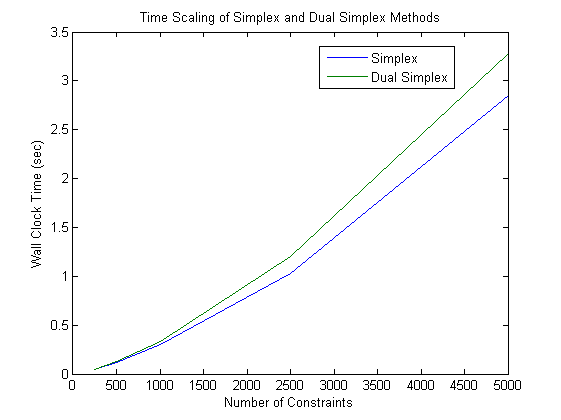
\includegraphics{../plot/figs/fig_simplex_time.png}
	\caption{Wall-Clock Times for Simplex and Dual Simplex}
	\label{fig:fig_simplex_time}
\end{figure}



\section*{Motivation}
%A classical formulation of the robust convex program is
%\begin{align}\label{RCP}
%\begin{split}
%\begin{aligned}
%    & \underset{x \in \mathcal{X}}{\text{minimize}}
%    & & c^T x \\
%    & \text{subject to}
%    & & f(x,\delta) \leq 0 \quad \forall \delta \in \Delta.
%\end{aligned}
%\end{split} \tag{RCP}
%\end{align}
%where $\mathcal{X} \subseteq \mathbb{R}^n$ is compact, $\Delta \subseteq \mathbb{R}^d$ is the uncertainty set, and $f:\mathcal{X} \times \Delta \mapsto \mathbb{R}$ is convex in $x$ for any fixed $\delta$.
%The problem \ref{RCP} involves an infinite number of constraints, and is therefore intractable in general

Another possible direction to look is to take $x^{**}$ as some convex combination of the
optimals solutions from the subproblems.  Intuitively, if each of the subproblems somehow
approximate \ref{CCP}, then somehow ``averaging'' them should give us at least something
no worse.

Ideally we would like to prove rigorous results about $x^{**}$.  How does the $x^{**}$
relate to the optimal solution of \ref{SCP}?  
Can we prove any results on the violation probability of $x^{**}$?
Alternatively, we could empirically evaluate the \ref{CCP} feasibility probabilities of $x^{**}$ 
via Monte Carlo simulation.
A recent paper by Carlone et al. \cite{carlone2014} looks to be related, but was discovered late and thus
we have not had time to properly review it.  We will thus perform a thorough literature review
to hone our research questions.

\section*{Experiments}
We intend to conduct experiments on the performance of the parallel procedure versus the traditional serial \ref{SCP} procedure.
For measures of performance of the solutions $x^*$ and $x^{**}$, we will look at the objective function values, the expected violation probabilities, and the probabilities that the violations probabilities are greater than $\epsilon$.
%For estimating the last two of these performance measures, we will use Monte Carlo simulation and test over problems for which one can explicitly characterize the feasible region of \ref{CCP}.
We will make comparisons based on both the total number of samples and the total wall-clock times of the two procedures.

We will also experiment with variations of the basic procedure.
One variation would involve communicating the support constraints of the master's problem back to the slaves and doing new sampling before solving new subproblems for each slaves.
This could be done over a number of iterations and we could study the performance of the returned solutions at each iteration.

Another variation would again involve communicating support constraints of the master's problem back to the slaves, but instead of doing new sampling, we re-solve the subproblems with the additional shared support constraints.
After sending the support constraints of these new subproblems to the master, we could perform one final solve and get a solution that is no worse than the previous.
This is because passing support constraints from the master to the slaves would allow for constraints that were not previously support constraints to become support constraints.

\bibliographystyle{siam}
\bibliography{references} 

\end{document}